\documentclass{beamer}

\usepackage{fontspec} 
\usepackage{lsp-makros}
\usepackage{rotate}

\useoutertheme{lsp}

\usepackage{ngerman}
\usepackage{lsptitle}
\usepackage{mdframed}
\def\two@digits#1{\ifnum#1<10 0\fi\number#1}
\def\mytoday{\two@digits{\number\day}.\two@digits{\number\month}.\number\year}


\usepackage{xspace,multicol}
\newcommand{\latex}{\LaTeX\xspace}
\usepackage{tikz}


\newcounter{lastpagemainpart}
\footnotesep0pt
\renewcommand{\footnoterule}{}
\usefootnotetemplate{
  \noindent
  \insertfootnotemark\insertfootnotetext}

\let\beamerfn=\footnote
\renewcommand{\footnote}[1]{%
\let\oldfnsize=\footnotesize%
\let\footnotesize=\tiny%
\beamerfn<\thebeamerpauses->{#1}%
\let\footnotesize=\oldfnsize}


\date{\today}

\usepackage{eurosym}  
 
\renewcommand{\centerline}[1]{\hfill#1\hfill\hfill\mbox{}}


\title{\mbox{Auf der Suche nach dem `Kunden'} \large Globaler Nutzen \& lokale Kosten}

% \institute{FU Berlin}
\author[LangSci]{Sebastian Nordhoff \& Debora Siller}


\newlength{\distlength}
\setlength{\distlength}{.7mm}

\newcommand{\saeule}[2][green]{
\raisebox{-.4cm}{\parbox{0cm}{\parbox{1cm}{\centering #2}}}\colorbox{#1}{\parbox[b][#2\distlength][b]{1cm}{\color{#1}\rule{1cm}{.3pt}}}
}

\newcommand{\distribution}[5]{
\parbox[b][.9\textheight][b]{\textwidth}{
  \centering 
\setlength{\fboxsep}{0pt}
\saeule[langscicol1]{#1}
\saeule[langscicol2]{#2}
\saeule[langscicol3]{#3}
\saeule[langscicol4]{#4}
\saeule[langscicol5]{#5}
}
}
 



\begin{document}
\lspbeamertitle
\frame{ 
\frametitle{Outline}
\tableofcontents
}

\section{Einleitung}
\frame{ 
\frametitle{Language Science Press} 
\begin{itemize}
  \item aktiv seit 2014, Anschubfinanzierung durch DFG
    \begin{itemize}
    \item Förderungsbedingung: Entwicklung eines Geschäftsmodells
    \end{itemize}
 \item nur Bücher, nur Spitzenforschung, nur Sprachwissenschaft
 \item international, reihenbasiert
 \item 9 veröffentlichte Bücher, >100 Interessensbekundungen
 \item 16 Reihen 
 \item Bücher zwischen 100 und 800 Seiten
%  \item Tieferes technisches Verständnis kann bei den Autoren nicht vorausgesetzt werden
 \item http://www.langsci-press.org 
\end{itemize} 


}
 



      \frame{ 
\frametitle{\raggedright Globaler Nutzen, lokale\\ Kosten und Jurisdiktion}
 

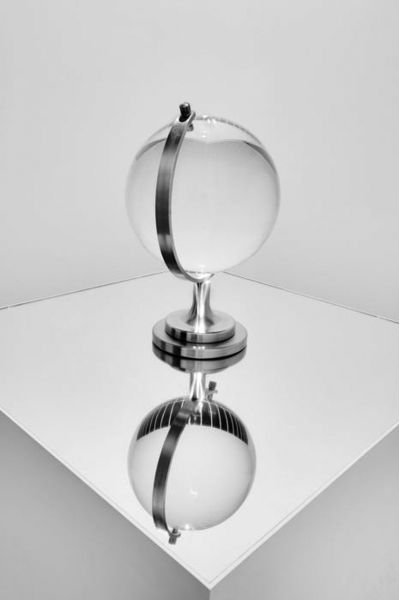
\includegraphics[height=.95\textheight]{pics/globe.jpg}~
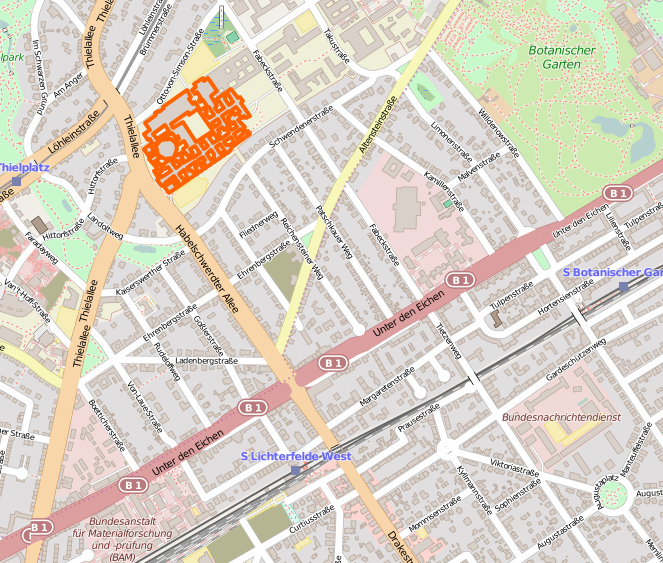
\includegraphics[height=.95\textheight]{pics/silberlaube.png}

{~\\
\tiny 
CC-BY-SA; ODbL  OpenStreetMap Foundation \\ 
CC-BY-SA https://commons.wikimedia.org/wiki/File:Melik\_Ohanian\_Futuring\_\%28Planet\%29\_2011.jpg
} 

}



\section{Kosten}
\frame{ 
\frametitle{Geschäftsmodell} 
\begin{itemize}
 \item Vision: wo wollen wir hin?
 \item Akteure: wer kommt mit? 
 \item Kosten: was kostet das?
 \item Einnahmearten: wie kriegen wir das Geld wieder rein?
%  \item Berechnungen
\end{itemize} 
}

 
\frame{ 
\frametitle{Kosten}
\begin{columns}
\column{6cm}
\begin{itemize}
 \item Personal 
 \item Sachkosten
\end{itemize}
   \begin{itemize}
 \item    Derzeit ca. 10k€/Buch
\item perspektivisch 3,5k€
\item {\LaTeX}-Satz autorenseitig
 \item Bei 50 Büchern/Jahr:
\begin{itemize}
 \item  150k€ Personalkosten
 \item  40k€ Sachkosten
\end{itemize} 
\end{itemize}
\column{4cm}
\setlength\distlength{.3mm}
\saeule[langscicol1]{150}
\saeule[langscicol2]{40}
\end{columns}
}



\frame{ 
\frametitle{Kostenverteilung} 
\begin{itemize}
 \item Autorenbetreuung 40\% 
 \item Herausgeber-Betreuung 8\%
 \item long tail: Feinsatz, Koordinierung PoD, Ausstattung, IT, Design, Marketing, Reise, Rechtsberatung, Steuerberatung, Verbrauchsmaterialien, Dokumentation,  strategische Planung, Mittelakquise, \dots	
\end{itemize}

\medskip
\vspace*{.2cm}
\hspace*{.7cm} 
\saeule[langscicol1]{40}
\saeule[langscicol2]{8}
\saeule[langscicol3]{6}
\saeule[langscicol4]{5}
\saeule[langscicol5]{5} 
\saeule[langscicol6]{4} 	
}
 
    
\frame{ 
\frametitle{\mbox{Vergleich zu Kosten anderer} Verlage}
\begin{itemize}
 \item geringe Kosten
\begin{itemize}
 \item Rechtsberatung: keine komplizierten Autorenverträge durch CC-BY 
 \item IT: keine aufwendige Zugangskontrolle, kein DRM, keine Rechnungslegung
 \item http://bjoern.brembs.net/2014/07/are-we-paying-us3000-per-article-just-for-paywalls/
\end{itemize} 
 \item kalkulatorische Schätzwerte können nach dem Vortrag eingesehen werden   
\end{itemize}

}

     

\section[Stakeholder]{Stakeholder: auf der Suche nach dem `Kunden'}
 
\frame{ 
\frametitle{Stakeholder} 

\begin{itemize}
 \item Ein Kunde bezahlt etwas und erhält dafür eine Gegenleistung
\end{itemize}


\begin{itemize}
 \item  Autoren \pause
 \item  Leser \pause
 \item  Bibliotheken \pause 
 \item  Universitäten  \pause
 \item  Fachgesellschaften  \pause
 \item  (Staat)  \pause
\end{itemize} 

\begin{itemize}
 \item \textbf{Bezahler und Nutznießer fallen nicht unbedingt zusammen} 
 \item Wer ist der `Kunde'? Wer zahlt? 
\end{itemize}

} 
 

\section{Wertversprechen}
\frame{ 
\frametitle{Wertversprechen}
\begin{tabular}{lll}
 \onslide<1-7> Autoren  & $\to$ &  \onslide<2-7>Sichtbarkeit, Karma\\
 \onslide<1-7> Leser  & $\to$ &  \onslide<3-7>Zugang, Nachnutzung\\
 \onslide<1-7> Bibliotheken   & $\to$ &  \onslide<4-7>Zugang zu Wissen, Kostensenkung\\
 \onslide<1-7> Universitäten   & $\to$ &  \onslide<5-7>Schaffung von Wissen, Kostensenkung \\
 \onslide<1-7> Fachgesellschaften   & $\to$ &  \onslide<6-7>Förderung wissenschaftlichen Austausches\\
 \onslide<1-7> (Staat)   & $\to$ &  \onslide<7>Volksbildung, Kostensenkung
\end{tabular}
}
 
\section{Einnahmearten}

\frame{ 
\frametitle{Einnahmearten} 
\begin{enumerate}
 \pause\item  Publikationsgebühren 
 \pause\item  Individualmitgliedschaften 
 \pause\item  institutionelle Mitgliedschaften 
 \pause\item  Spenden 
 \pause\item  Printmarge 
 \pause\item  (staatliche Grundfinanzierung)
\end{enumerate} 
\pause
Je mehr Einnahmearten, desto mehr Verwaltungsaufwand!
}

\frame{ 
\frametitle{Publikationsgebühren}
\begin{columns}
\column{5cm}
\begin{itemize}
 \item Gruppe \textbf{Autor}
 \item Höhe 3500€
 \item no-questions-asked-waiver
 \item Falls Autoren Zugang zu Fördermitteln haben, sollte man diese nicht verfallen lassen
\end{itemize} 
\column{5cm}
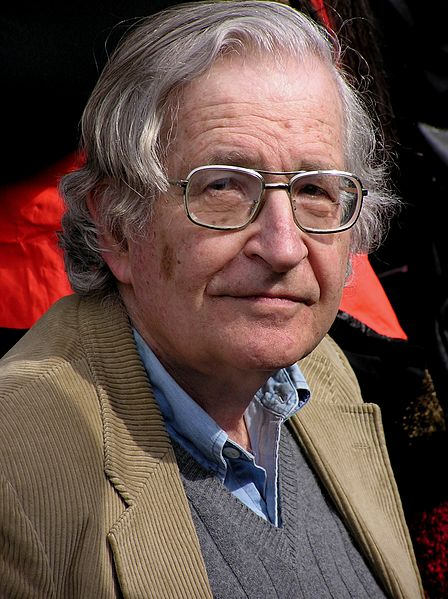
\includegraphics[width=4cm]{pics/Chomsky.jpg}
\\
\tiny 
CC-BY Duncan Rawlinson
http://flickr.com/photos/thelastminute/97182354/in/set-72057594061270615/
\end{columns}
}
 
 
\frame{ 
\frametitle{Fördermitgliedschaften} 
\begin{columns}
\column{5cm}
\begin{itemize}
\item Gruppe \textbf{Leser}
\item regelmäßige Förderung mit frei wählbarem Betrag
\item vorgeschlagen: 30€/Jahr
\end{itemize} 
\column{5cm}
% 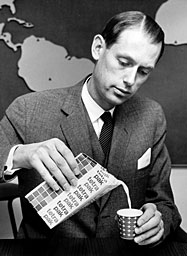
\includegraphics[width=4cm]{pics/rausing.jpg}
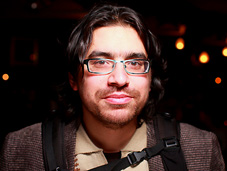
\includegraphics[width=4cm]{pics/harald.jpg}\\
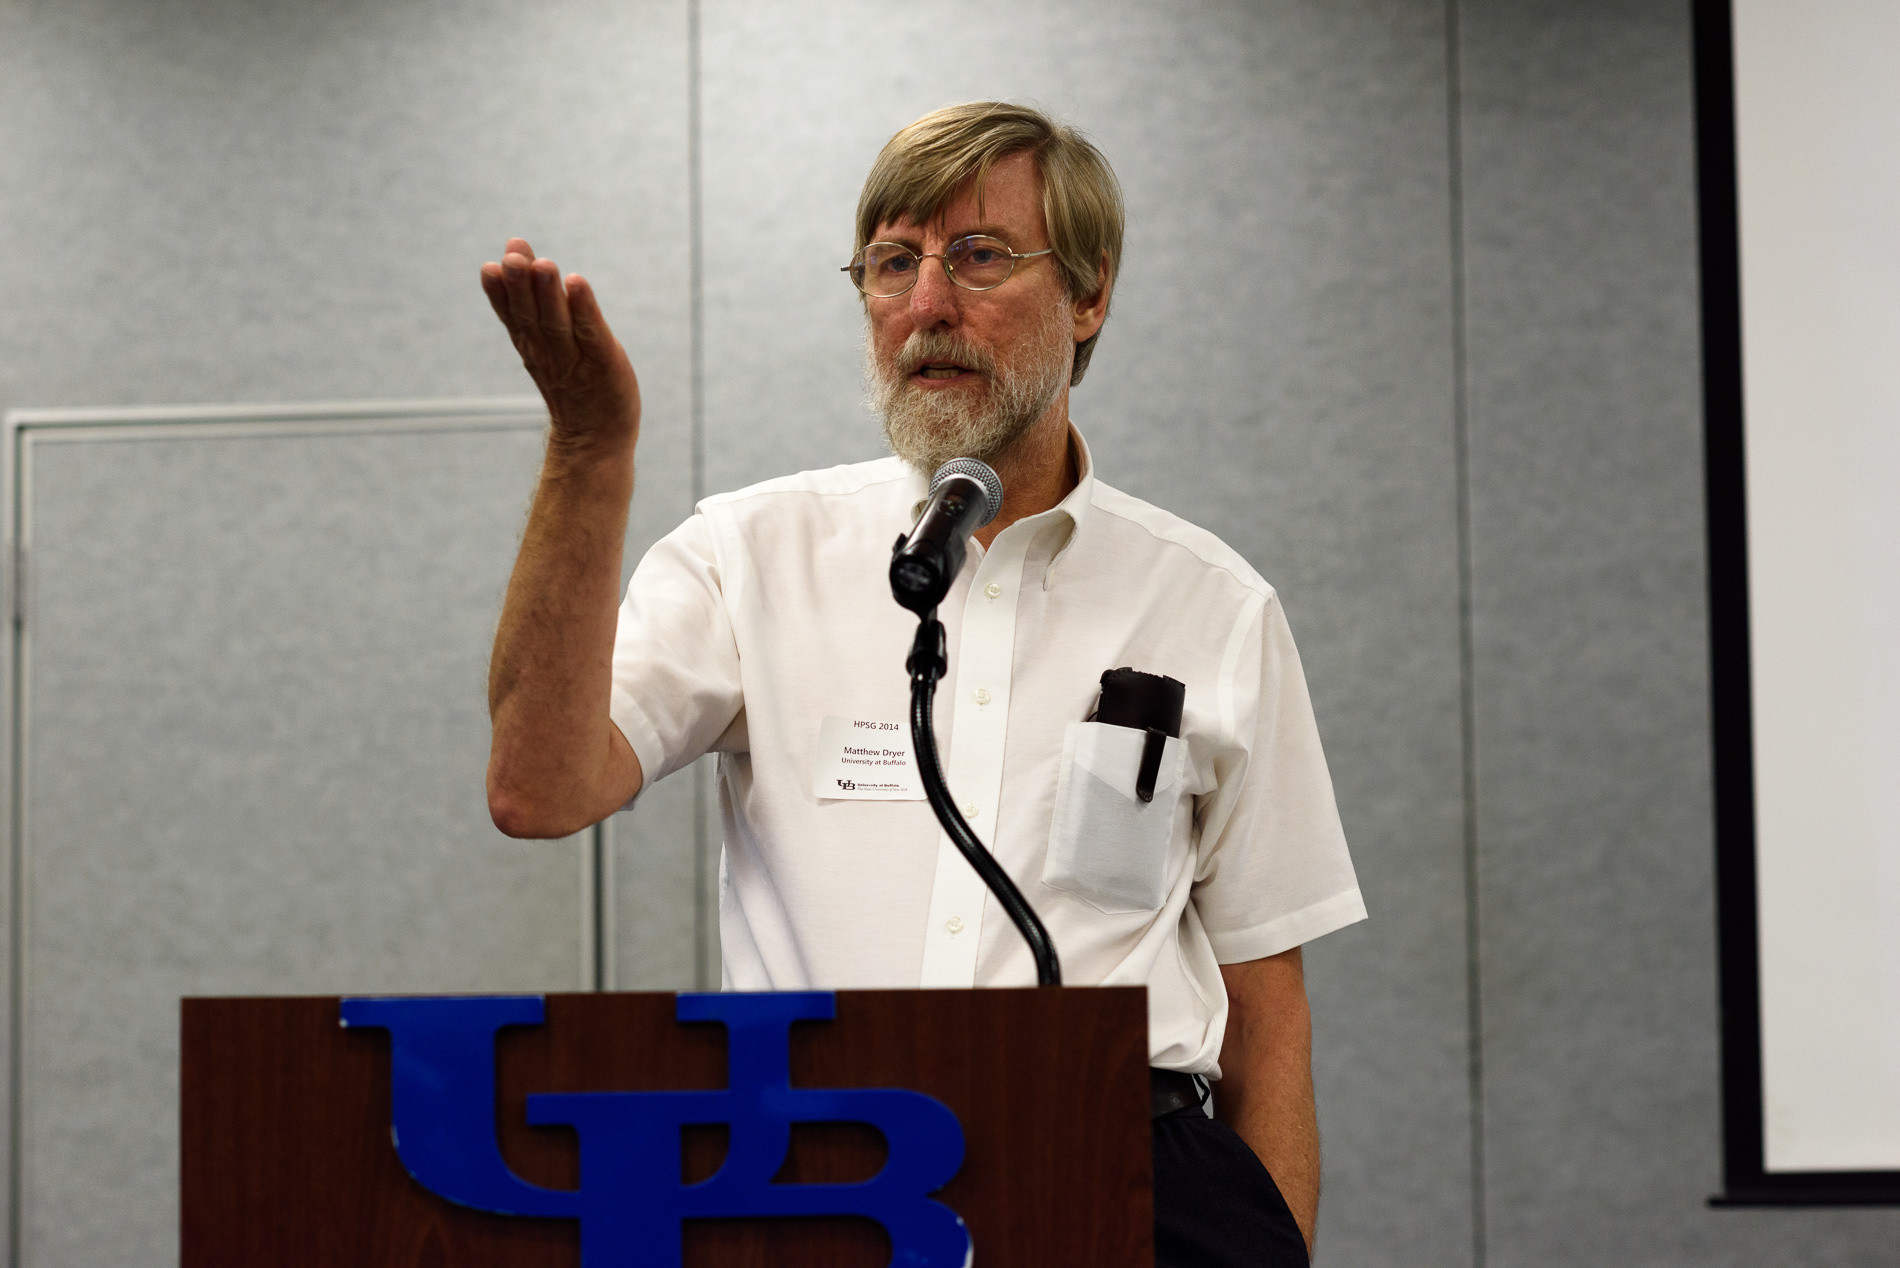
\includegraphics[width=4cm]{pics/dryer.jpg}\\[2.3em]
\hspace*{-5.5cm}
\parbox{2\textwidth}{\tiny 
CC-BY-NC-ND Stefan Müller\\[-.3em] 
http://hpsg.fu-berlin.de/~stefan/Bilder/wp-content/gallery/matthew-dryer\_1/20140827-23-34-38.jpg}
\end{columns}
% rausing

}

 
\frame{ 
\frametitle{Institutionelle \mbox{Mitgliedschaften}} 
\begin{columns}
\column{5cm}
\begin{itemize}
 \item Gruppe \textbf{Universitäten}; \textbf{Bibliotheken}
 \item gestaffelte Preise nach Größe der Institution und Wirtschaftskraft des Landes 
 \item Modell von OpenLibHums, Arxiv
\end{itemize} 
\vspace*{1.5cm}
\column{5cm}
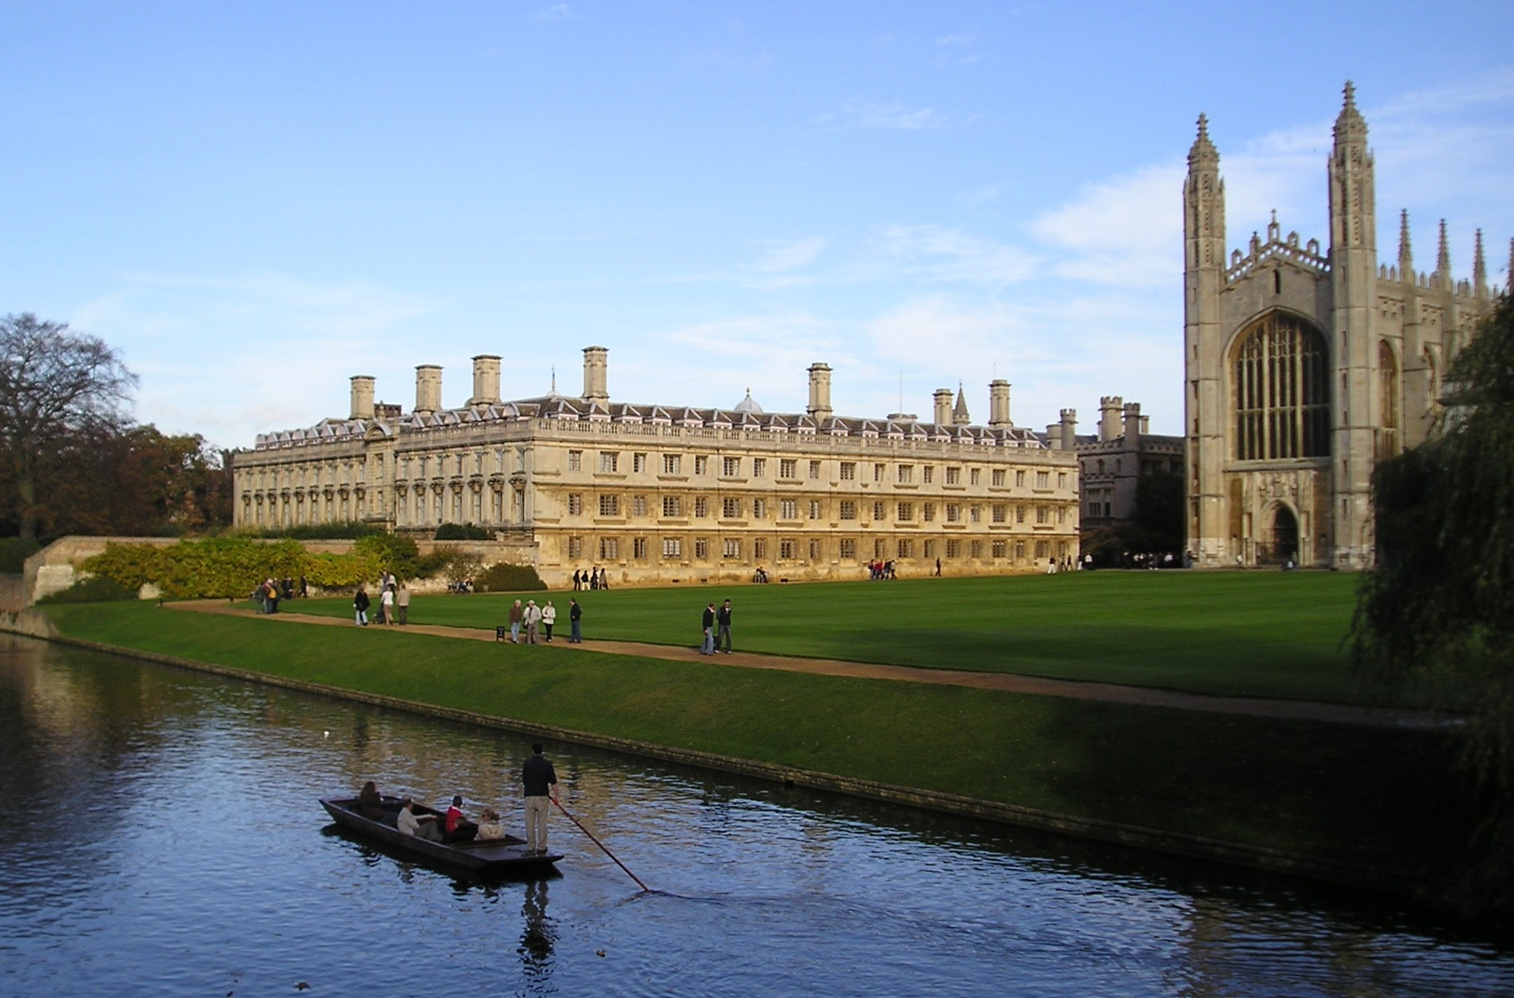
\includegraphics[width=4cm]{pics/cambridge.jpg}\\
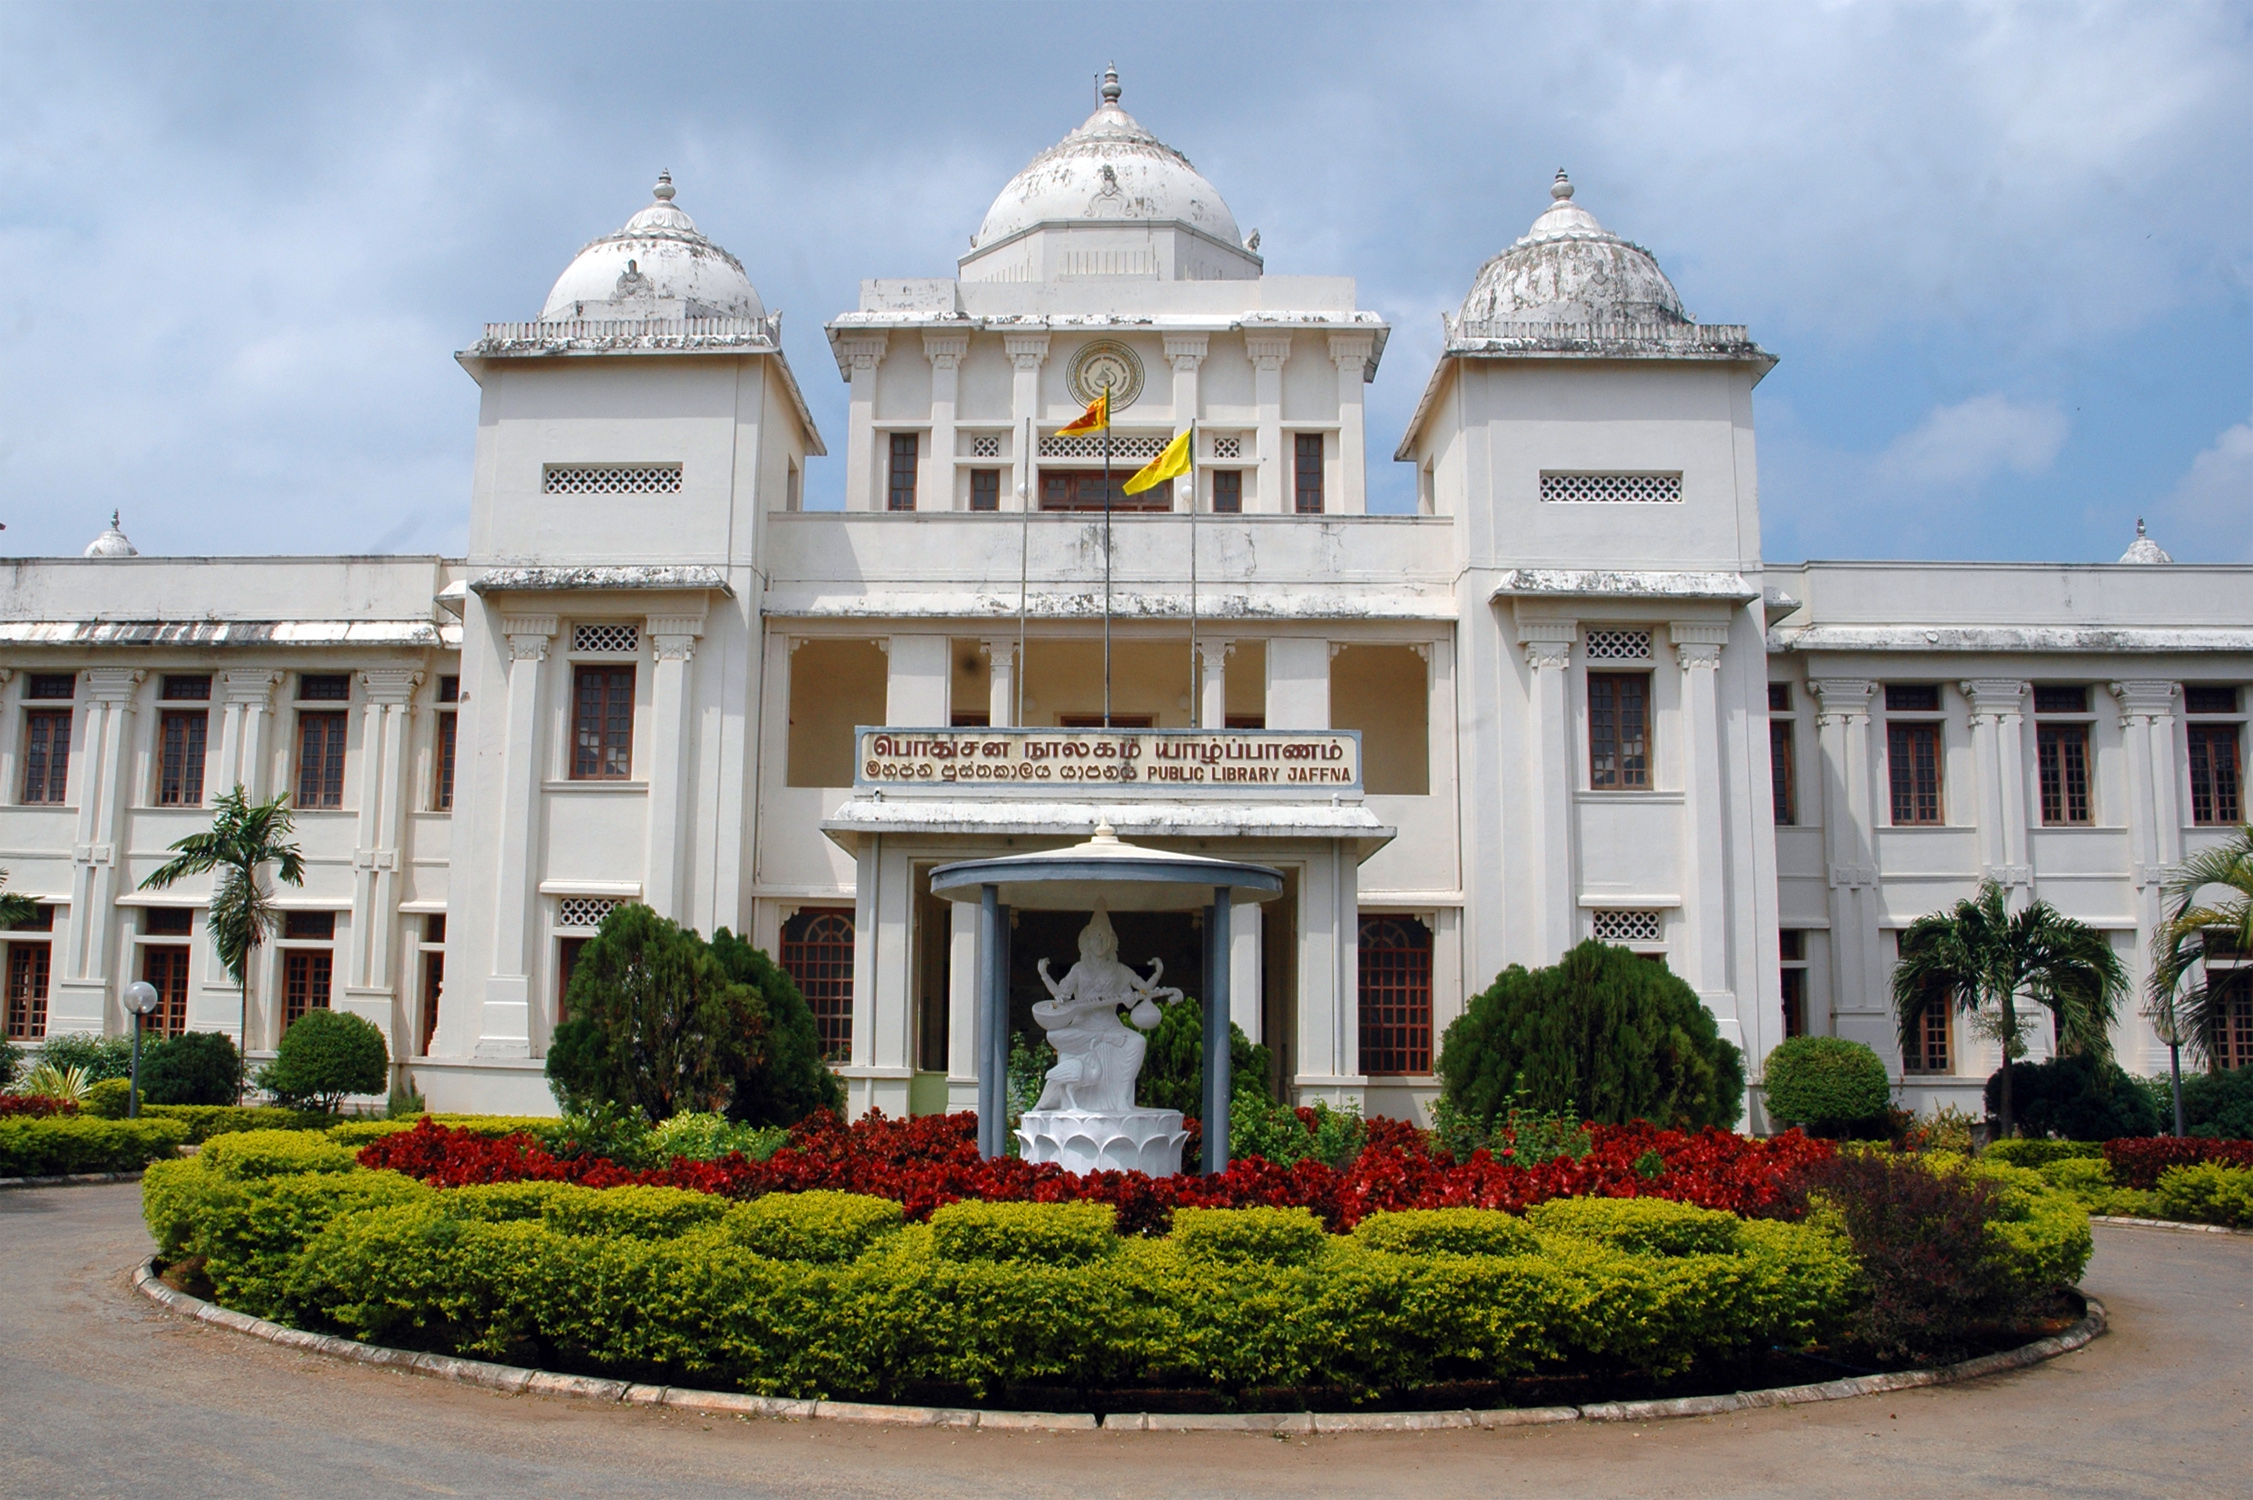
\includegraphics[width=4cm]{pics/jaffna.jpg}\\[3.3em]
\hspace*{-5.5cm}
\parbox{2\textwidth}{\tiny 
 CC-BY-SA Christian Richardt {https://de.wikipedia.org/wiki/Datei:ClareCollegeAndKingsChapel.jpg}\\[-.1em]
CC-BY-SA Anton Croos  https://de.wikipedia.org/wiki/Datei:Public\_Library,\_Jaffna.JPG}
\end{columns} 
}

 
\frame{ 
\frametitle{Spenden} \vspace*{1cm}
\begin{columns}
\column{5cm}
\begin{itemize}
 \item Gruppe \textbf{Leser}; \textbf{Autoren}
 \item einmalige Förderung mit beliebigem Betrag 
 \item steuerlich absetzbar
\end{itemize} 
\vspace*{2cm}
\column{5cm} 
\vspace*{2cm}

\includegraphics[width=4cm]{pics/spardose.jpg}\\ 
\hspace*{-5.5cm}
\parbox{2\textwidth}{\tiny 
 CC-BY-NC \\[-.3em]
https://www.flickr.com/photos/sarahamina/4510470695/in/photolist-3J6EhQ-agwAjL-88vZmn-7SzkWv-7SCC4E-7SzkN8-dazm1i-Q2Ec2-4uPzV6-4uTAqh-5pWZZL-7oG5C5-iGdNBU-qV4kMC}
\end{columns}  
% spardose


}

 
\frame{ 
\frametitle{Printmarge}  
\begin{columns}
\column{5cm}
\begin{itemize}
 \item Gruppe \textbf{Leser}; \textbf{Bibliotheken}
 \item Kalkuliert: 10€ Nettomarge pro PoD-Buch
 \item Endkosten pro Buch: 30--60€
\end{itemize} 
\column{5cm}

\includegraphics[width=4cm]{pics/enfield.png}
\end{columns} 
}
 
 
\frame{ 
\frametitle{(staatliche Grundfinanzierung)}  
\begin{columns}
\column{7cm}
\begin{itemize}
 \item Nicht Teil dieses Geschäftsmodells
 \item Begründung: Verbreitung von Forschungsergebnissen sollte eine hoheitliche Aufgabe sein
\end{itemize} 
\column{5cm}
~~~
\includegraphics[width=2cm]{pics/bundesadler.png}
\end{columns} 

}

\frame{ 
\frametitle{\mbox{Kosten- und Einnahmeberechnung}}
\begin{itemize}
 \item ca. 40 Variablen 
 \item \textbf{bekannt}: Tariftabellen, Steuersätze, Supporter
 \item \textbf{gut schätzbar}: Aufwand einzelner Arbeitschritte, Einreichungszahlen 
 \item \textbf{unbekannt}: Spendenbereitschaft, Fördermitgliedschaften, Autorengebührenquote
\end{itemize}
} 
 


\section{Einnahmeverteilung}

\frame{ 
\frametitle{Einnahmeverteilung}  
\distribution{20}{20}{20}{20}{20}
}

\frame{ 
\frametitle{Einnahmeverteilung}   
\distribution{25}{30}{15}{10}{20}
}

\frame{ 
\frametitle{Einnahmeverteilung}    
\distribution{10}{80}{0}{5}{5}
}
\frame{ 
\frametitle{Einnahmeverteilung}   
\distribution{13}{24}{18}{29}{16}
}
 
\frame{ 
\frametitle{Einnahmeverteilung: so nicht}
\distribution{0}{0}{0}{0}{0}
}

\frame{ %berechnet nach xls
\frametitle{\mbox{Angenommene Verteilung für 2020}}
\distribution{29}{21}{32}{6}{14}\\[.4em]
\hspace*{2cm}
\parbox{1cm}{\centering\tiny Publikations\-gebühren}\hspace*{.3cm}
\parbox{1cm}{\centering\tiny Förder\-mitglieder}\hspace*{.3cm}
\parbox{1cm}{\centering\tiny Institutionelle Mitglieder}\hspace*{.3cm}
\parbox{1cm}{\centering\tiny Spenden\\~}\hspace*{.3cm}
\parbox{1cm}{\centering\tiny Printmarge\\~}
% \saeule[langscicol1]{29}\parbox{0cm}{\raisebox{-2cm}{\hspace*{-1cm}\rotate{\hspace*{-1cm}PubGeb}}}
% \saeule[langscicol2]{21}\parbox{0cm}{\raisebox{-2cm}{\hspace*{-1cm}FM}}
% \saeule[langscicol3]{32}\parbox{0cm}{\raisebox{-2cm}{\hspace*{-1cm}IM}}
% \saeule[langscicol4]{6}\parbox{0cm}{\raisebox{-2cm}{\hspace*{-1cm}SP}}
% \saeule[langscicol5]{14}\parbox{0cm}{\raisebox{-2cm}{\hspace*{-1cm}PM}}
 

% Publikationsgebühren 29
% Fördermitgliedschaften 21
% Institutionelle Mitgliedschaften 32
% Spenden 6
% Printmarge  14
}


\frame{ 
\frametitle{Evaluation} 
\begin{itemize}
 \item Die derzeitigen Annahmen sind ungenau
 \item Nachjustierung, sobald genauere Zahlen verfügbar werden
 \item Eventuell Anpassung der Strategie
\end{itemize} 
} 
  

\section{Rechtliches}



%       \frame{ 
% \frametitle{\raggedright Globaler Nutzen, lokale\\ Kosten und Jurisdiktion}
% \begin{itemize} 
%  \item  können wir Spendenbescheinigungen nach norwegischem Recht ausstellen?
%  \item  sind anonyme Spenden via Flattr o.\,ä.\ mit deuschen Verwaltungsvorschriften vereinbar?
%  \item  wie können Printmargen verbucht werden, wenn diese vom Dienstleister in den USA in USD angewiesen werden, bei der Uni aber in EUR ankommen und der Dienstleister sich weigert, die Kostenstelle in den Betreff der Überweisung zu schreiben?
% \end{itemize}
% $\Rightarrow$     ab welcher Höhe deckt eine Spende ihren Verwaltungsaufwand?
%    \begin{itemize}
%  \item    Reduzierung des Verwaltungsaufwandes durch Gründen eines Fördervereins
% \end{itemize}
% }
 
\frame{ 
\frametitle{Nachhaltigkeit}
\begin{itemize}
 \item Die Unternehmung sollte agil handeln können
 \item Die Unternehmung soll betriebswirtschaftlich verantwortlich handeln 
 \item Die Unternehmung soll kostendeckend arbeiten
 \item \textbf{Die Rechtsform sollte auf keinen Fall profitorientiert sein}
  \begin{itemize}
    \item Verkauf von Prestige 
    \item Bei Erfolg: Profitmaximierung $\to$ Anhebung der Preise
  \end{itemize}
%  \item gewählte Rechtsform: {\glqq}Betrieb gewerblicher Art{\grqq} an der Freien Universität Berlin
\end{itemize}
}

\section{Übertragbarkeit}


\frame{ 
\frametitle{Offen heißt offen}
\begin{itemize}
 \item Autoren behalten ihr Copyright
 \item Alle Werke stehen unter freier Lizenz nach opendefintion.org (CC-BY)
 \item Quellcodes aller Bücher und Softwarebestandteile  sind vollständig auf github zur Nachnutzbarkeit verfügbar
 \item Betriebswirtschaftliche Zahlen werden veröffentlicht, sobald diese belastbar vorliegen
 \item Geschäftsprozesse werden in geeigneter Weise zur Nachnutzung bereitgestellt (z.\,B.\ heute)
\end{itemize}
% \column{5cm}
% \includegraphics{}
% \end{columns}
}



\frame{ 
\frametitle{Übertragbarkeit}
\begin{itemize}
 \item scholar-owned publishing 
    \begin{itemize}
    \item starke Markenbildung; Marke nicht im Besitz profitorientierter Unternehmen
    \end{itemize}
 \item autarkes Reihenmodell 
 \item Einbindung der Community
 \item Finanzierungskonzept grundsätzlich übertragbar
    \begin{itemize}
      \item allerdings wohl demnächst heißer Wettkampf um Födermitgliedschaften (oder Kooperation)
    \end{itemize}
 \item kalkulatorische Zahlen als Grundlage für ähnliche Projekte, sobald empirisch unterfüttert
\end{itemize}
}



\section*{Danke}

\frame{ 
\frametitle{Vielen Dank}
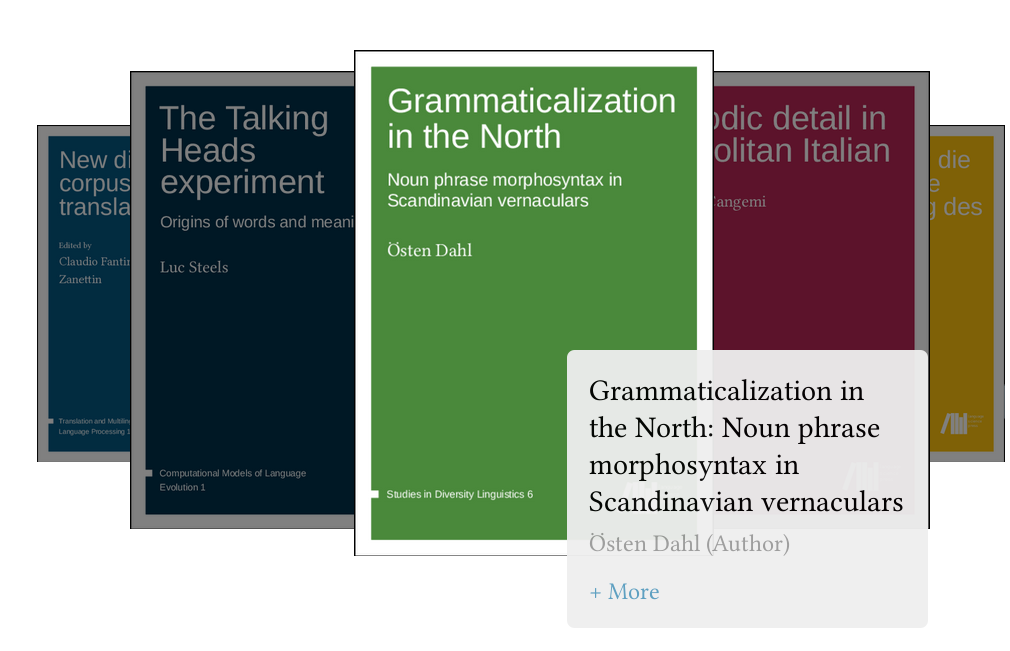
\includegraphics[height=1\textheight]{pics/catalog.png}
}

% OLH
% Edition Open Access
 
\end{document}


https://www.flickr.com/photos/librarygeek/4503670035/
geschuhn